\chapter{AWS Deployment \\
\small{\textit{-- Matthew Smith, Bowen Jiang, Gleb Myshkin}}}
\index{awsdeployment} 
\index{Chapter!AWS_Deployment}
\label{Chapter::AWS_Deployment}


\section{Digital Ocean Web Deployment (Instead of AWS)}
Website Link: \href {https://color-buttons-app-eg5ye.ondigitalocean.app}{https://color-buttons-app-eg5ye.ondigitalocean.app}

We tried to use Amazon AWS but we had issues along the way and decided to use Digital Ocean as it seemed to be easier to use and we'll be working with it later on. We did not have a step-by-step guide on how to take the button website and put it into Digital Ocean in order to access the website on the cloud, without having Docker constantly running on the operating system. So, we had some help with ChatGPT and Gemini to get the code in order to take the website code and push it to Digital Ocean with the help of Docker. The code below hasare the lines that were used in Windows Powershell in order to get the website running correctly. There are comments that describe what was the purpose of each line of code. The code below was the used in the same order as it is written. The website link is located at the very beginning of this section.

\begin{lstlisting}[style=linuxstyle, language=bash]
#ChatGPT & Gemini was used to get the following code (comments not included):

#Authentication of doctl (use DigitalOcean API Token created in DigitalOcean)
doctl auth init

#Creation of the Container Registry with the name of team-mgb-web-access and a basic tier subscription
doctl registry create team-mgb-web-access --subscription-tier basic

#Login to Docker (this is where the website is located on, with the use of DigitalOcean for cloud service)
doctl registry login

#Build Docker Image for the website
docker build -t color-buttons:v1 .

#Tag the image for the registry using registry name
docker tag color-buttons:v1 registry.digitalocean.com/team-mgb-web-access/color-buttons:v1

#Push the image to DigitalOcean
docker push registry.digitalocean.com/team-mgb-web-access/color-buttons:v1

#Verify if the upload was successful
doctl registry repository list team-mgb-web-access

#Added an app.yaml file to the folder where the website code is located, same place as the docker file, to tell DigitalOcean what to do with the Docker Image with the following code in it:
name: color-buttons-app
services:
- name: web
  image:
    registry_type: DOCR
    repository: color-buttons
    tag: v1
  http_port: 3000
  instance_size_slug: basic-xxs
  instance_count: 1

#Ran the app using the new app.yaml
doctl apps create --spec app.yaml

#The following code is the last one used to get the URL for the website
doctl apps list
\end{lstlisting}


\section{Change the Website}

\subsection{What Changed and Why}
The website in its original state used procedural JavaScript to add two event listeners directly to the buttons. The page background color received updates through separate handler functions for each button.

After the refactor, the logic was restructured into a \textbf{class-based design}.
A new class was introduced:

\begin{itemize}
  \item Identifying and storing references to the two button elements.
  \item Binding the click events to methods within the class.
  \item Providing a single method that updates the background color when called.
\end{itemize}

The webpage's appearance and user experience remained unchanged while maintaining their original layout. The code structure received an improvement through modular design, which enables better extension capabilities and follows object-oriented design principles.

\begin{figure} [H]
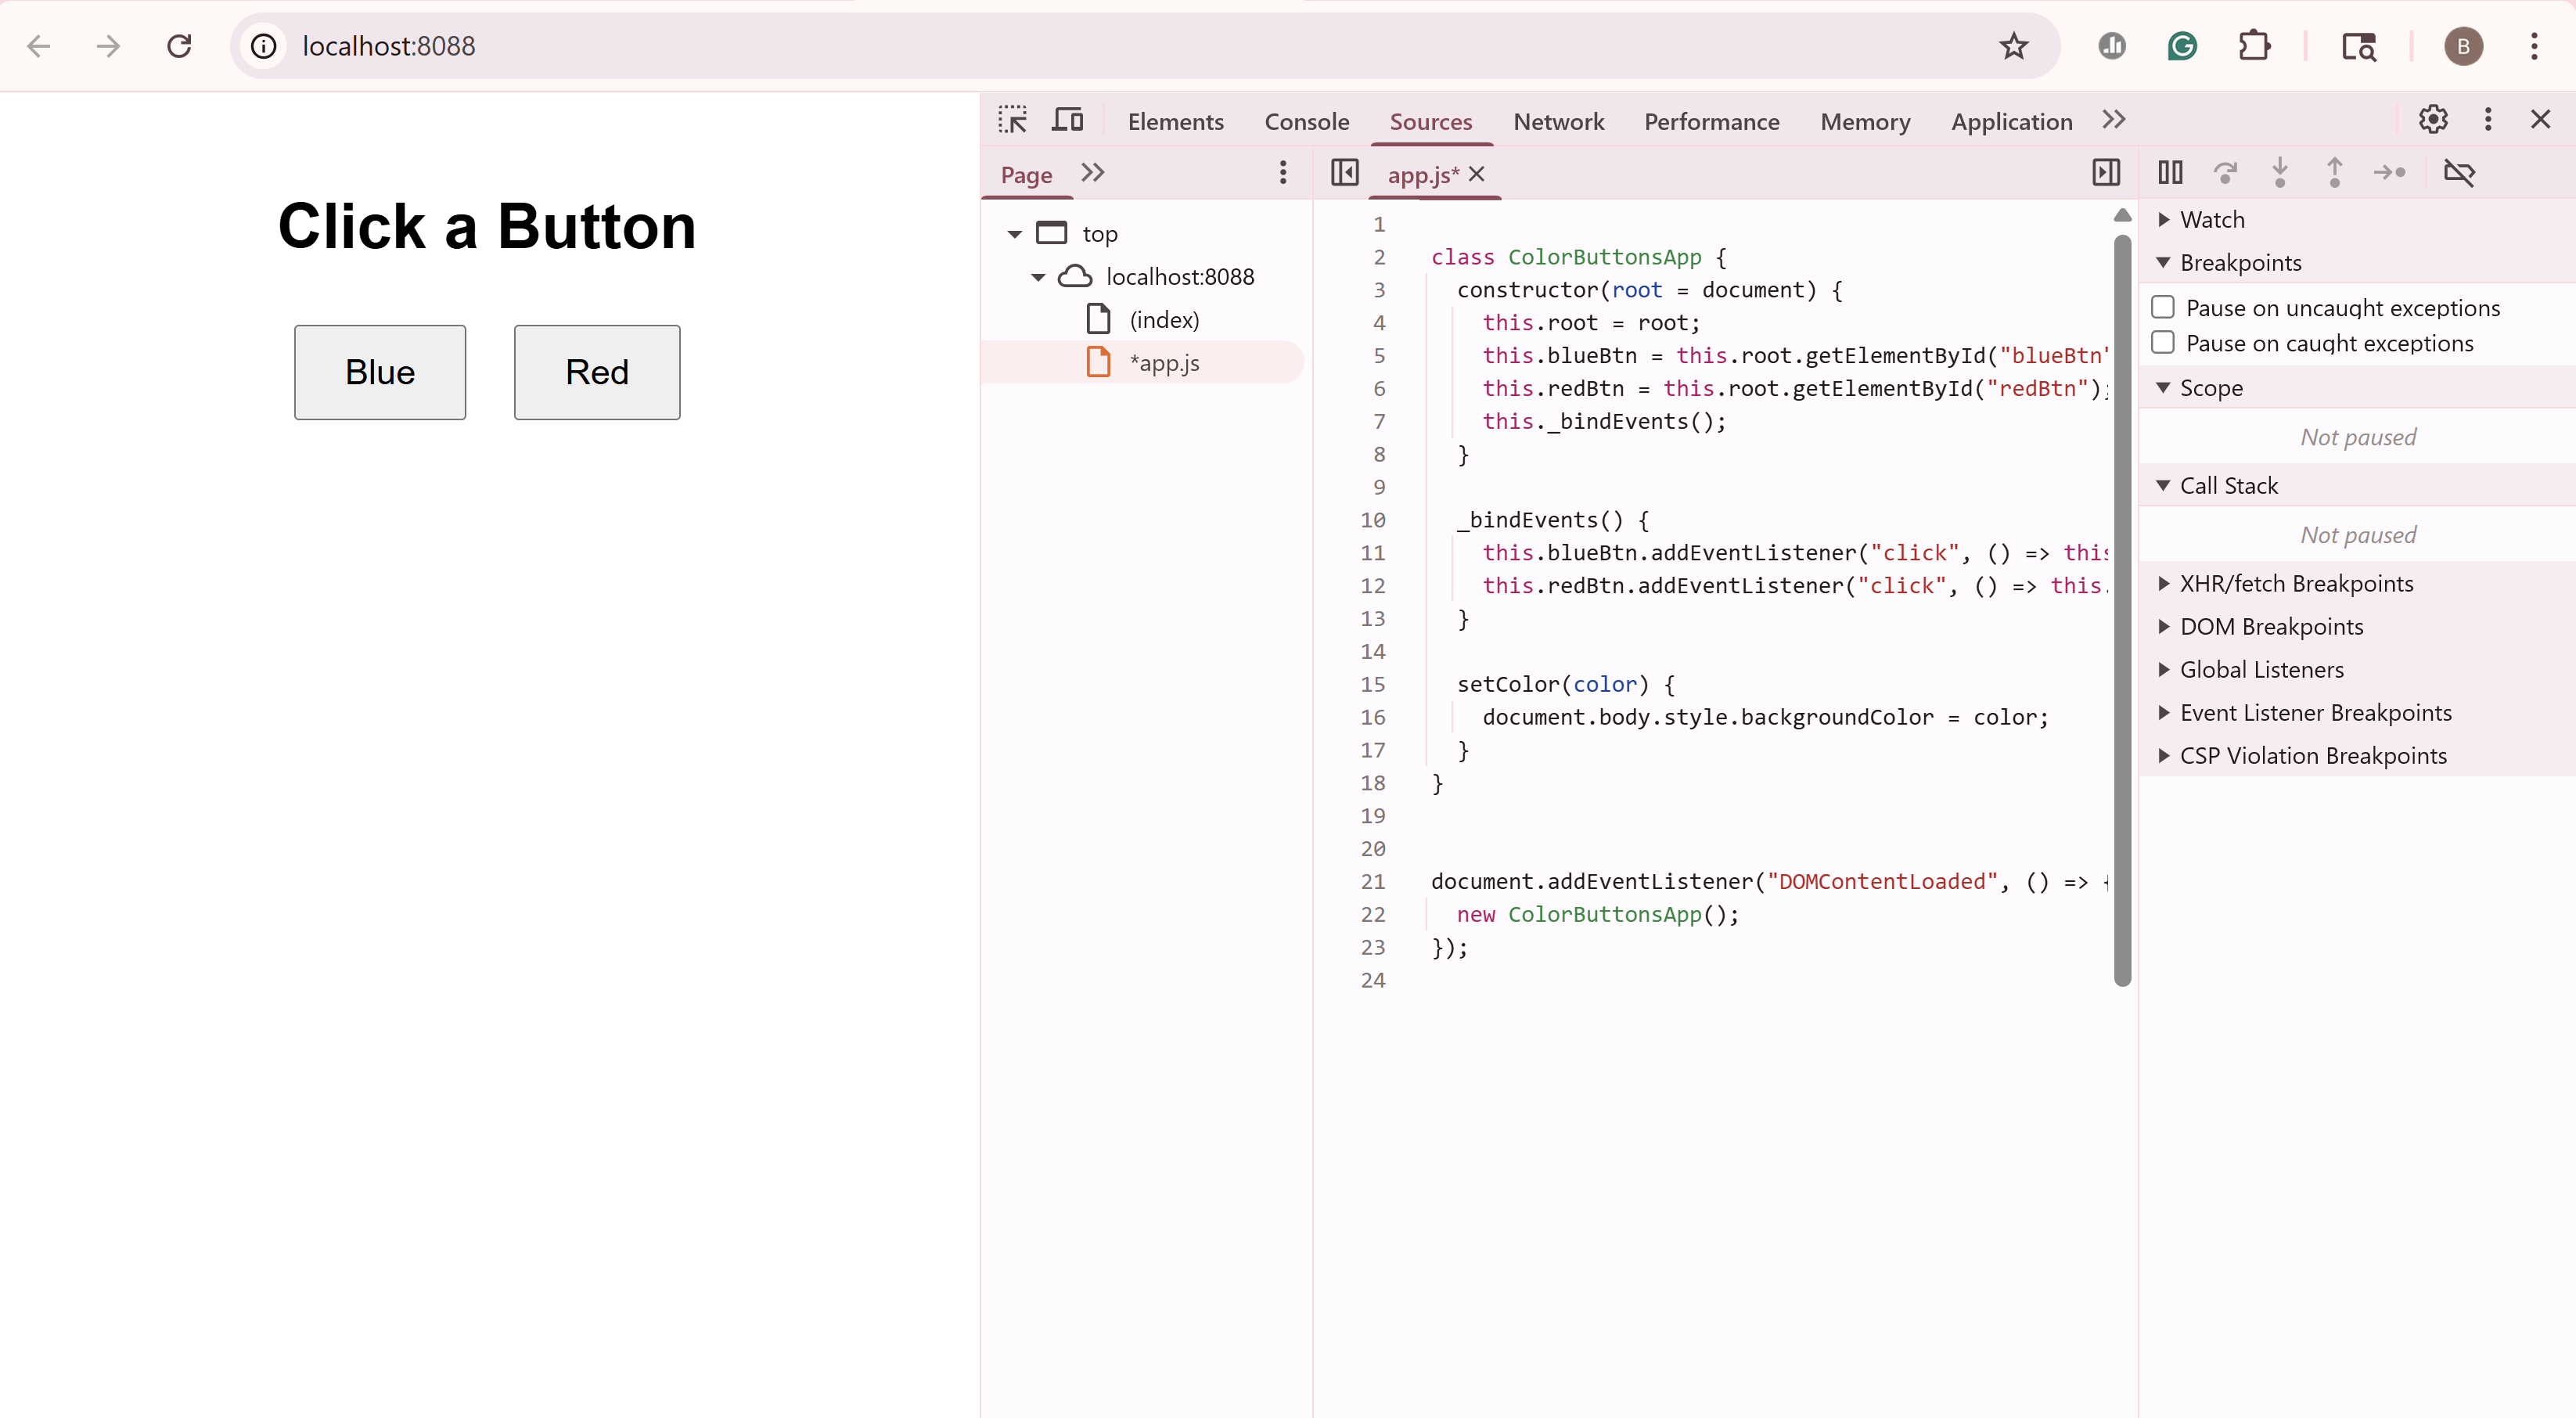
\includegraphics[width=\textwidth]{class .png}
  \centering
  \caption{Class-based JavaScript}
  \vspace{-0.3cm}
\end{figure}

\subsection{UML Class Diagram}
\begin{figure} [H]
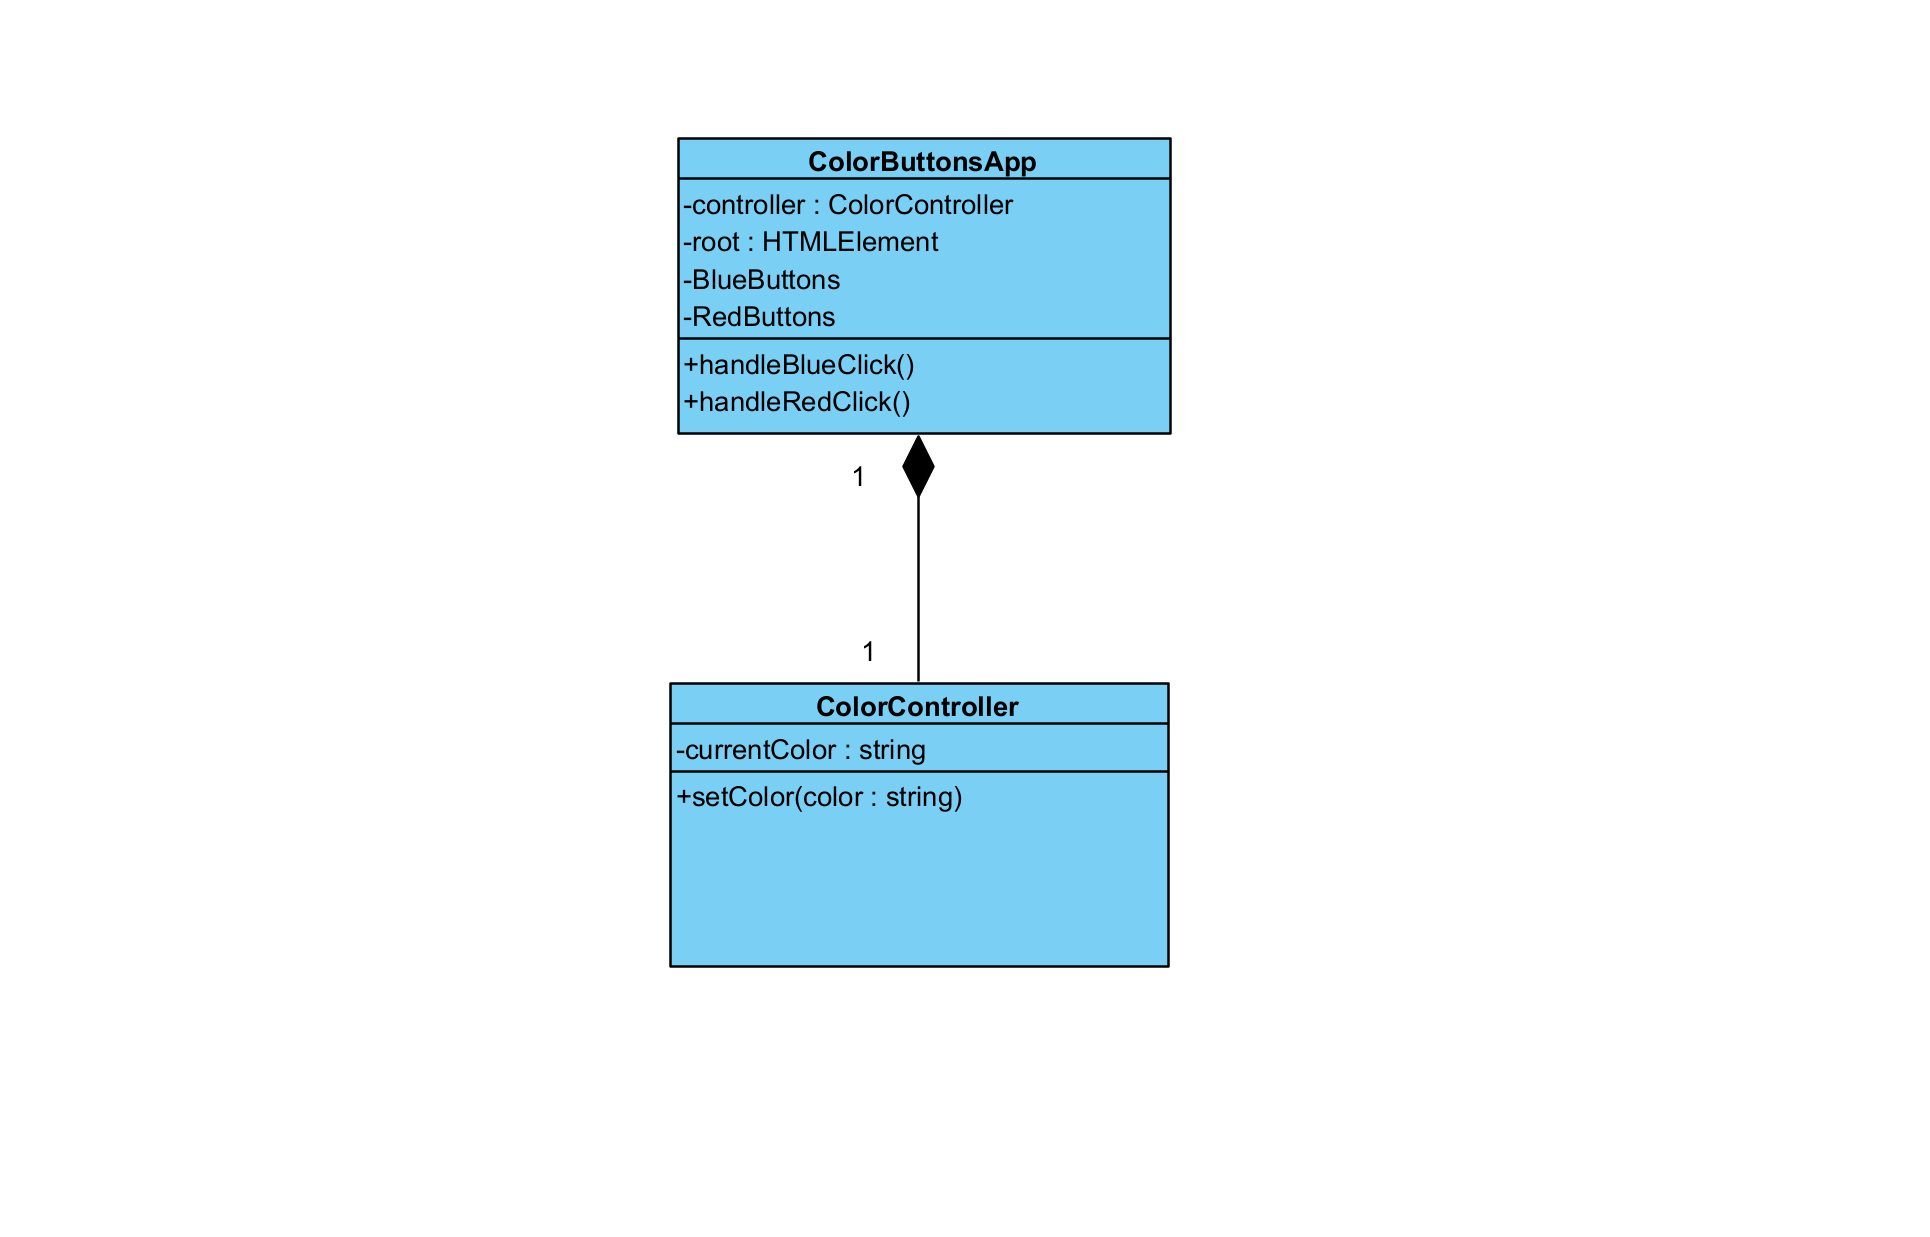
\includegraphics[width=\textwidth]{class diagram.png}
  \centering
  \caption{UML Class Diagram}
  \vspace{-0.3cm}
\end{figure}
